% File: basic_elements.tex
\documentclass{standalone}
\usepackage{pgfplots}
\pgfplotsset{compat=1.18}
\usepackage[american]{circuitikz}
\usepackage{cmbright}

\definecolor{myred}{RGB}{170,0,0}
\definecolor{myblue}{RGB}{0,0,220}
\definecolor{mygreen}{RGB}{0,150,0}
\definecolor{myorange}{RGB}{255,127,0}
% Brown
\definecolor{mybrown}{RGB}{150,75,0}

\ctikzset{bipoles/resistor/height=0.2}
\ctikzset{bipoles/resistor/width=0.5}
\ctikzset{bipoles/capacitor/height=0.4}
\ctikzset{bipoles/capacitor/width=0.15}

\begin{document}
% Simple RLC circuit, with equations, and plots of different quantities.
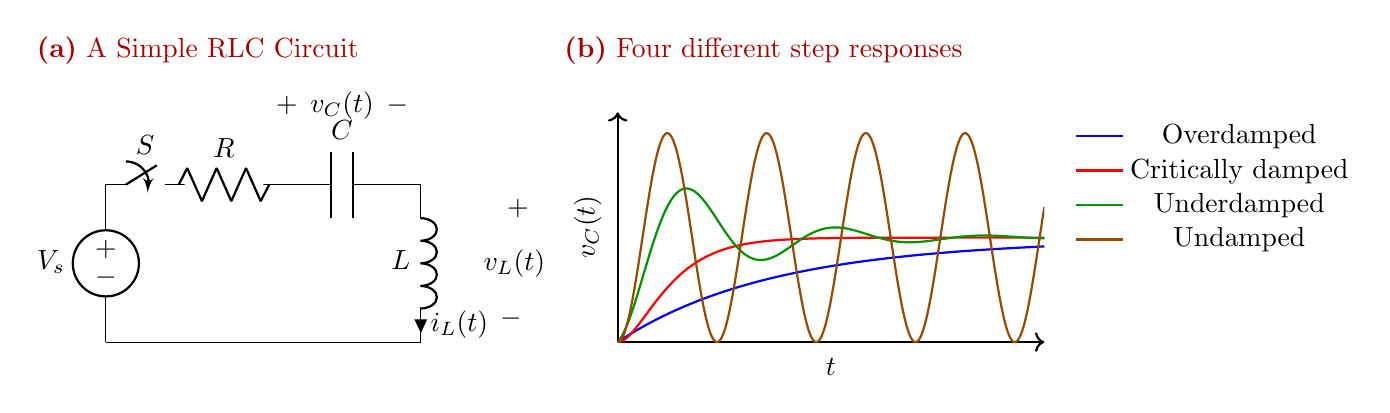
\begin{tikzpicture}
    % Subtitle for the circuit.
    \node[anchor=north west, color=myred] at (-1.0, 4.0) {\textbf{(a)} A Simple RLC Circuit};
    % --- Circuit (top left)
    \begin{scope}
        % Coordinates.
        \coordinate (A) at (4, 2);
        \coordinate (B) at (4, 0);
        \coordinate (L1) at (5.25, 2);
        \coordinate (L2) at (5.125, 0);
        \coordinate (C1) at (2, 3.0);
        \coordinate (C2) at (4, 3.0);

        % Voltage source and lower wire
       \draw (0, 0) to[V, l={$V_{s}$}, invert] (0, 2) to[closing
       switch, l=$S$] ++(1, 0) to[R, l=$R$] ++(1, 0) to[C, l=$C$] (A);
        \draw (0, 0) -- (B);

        % Inductor.
        \draw (A) to[L, l_=$L$, i^>=$i_L(t)$] (B);

        % Voltage label across capacitor
        \draw (C1) to[open, v^=$v_{C}(t)$] (C2);
        % Voltage label across capacitor
        \draw (L1) to[open, v^=$v_{L}(t)$] (L2);
    \end{scope}

    % Four different step responses of the circuit.
    \begin{scope}[xshift=6.5cm]
        \node[anchor=north west, color=myred] at (-0.8, 4.0) {\textbf{(b)} Four different step responses};
        \begin{axis}[
            width=7cm,
            height=4.5cm,
            xlabel={$t$},
            ylabel={$v_C(t)$},
            xmin=0, xmax=15,
            ymin=0, ymax=2.2,
            axis lines=left,
            axis line style={->},
            legend style={
                at={(1.05,1.0)},
                anchor=north west,
                draw=none,
                align=left
            },
            thick,
            samples=1000,
            domain=0:15,
            xtick=\empty,
            ytick=\empty
        ]

        % Overdamped: example with r1=2, r2=0.5
        \addplot[blue, thick] {1 - (0.8 * exp(-0.2*x) + 0.2 * exp(-0.1*x))};
        \addlegendentry{Overdamped}

        % Critically damped
        \addplot[red, thick] {1 - (1 + x) * exp(-x)};
        \addlegendentry{Critically damped}

        % Underdamped: damping ratio < 1
        \addplot[mygreen, thick] {1 - exp(-0.3*x) * cos(deg(1.2 * x))};
        \addlegendentry{Underdamped}

        % Undamped (LC circuit)
        \addplot[mybrown, thick] {1 - cos(deg(1.8 * x))};
        \addlegendentry{Undamped}

        \end{axis}
    \end{scope}
\end{tikzpicture}
\end{document}